\documentclass[conference]{IEEEtran}
\usepackage{tikz}
\usepackage{graphicx}
\usepackage{hyperref}

\begin{document}
\title{{Capability-Based Access Control Mechanisms:} \\ \centerline{\Large{A Survey and Implementation of Current Systems}}}

\author{
  \IEEEauthorblockN{Kritika Iyer}
  \IEEEauthorblockA{Cheriton School of Computer Science\\
    k4iyer@uwaterloo.ca}
  \and
  \IEEEauthorblockN{Sajin Sasy}
  \IEEEauthorblockA{Cheriton School of Computer Science\\
    ssasy@uwaterloo.ca}
  \and
  \IEEEauthorblockN{Justin Tracey}
  \IEEEauthorblockA{Cheriton School of Computer Science\\
    j3tracey@uwaterloo.ca}
    

}

\date{}


\maketitle
\begin{abstract}
Access control lists (ACL) are struggling to maintain the performance in systems, as the requirement for scalability in these systems increases. ACLs lead to higher overheads which in turn leads to inefficiency as the number of clients in the system increases. A distinct approach to address access control of resources is by using \textit{capabilities}. Capabilities are used to monitor access control on a per-client level, rather than on a per-resource level. As systems are becoming more distributed, capability based access control is appearing to be a closer fit to such systems, in comparison to ACLs.

Currently, there are multiple systems that implement capability-based resource management, both on user space and kernel space. But there are no established results that show that existing systems remain secure in the newly emerging paradigms. Most systems that are introduced in the latest research mostly have hypothetical constructions, but very few have actual implementations built. Those few which are implemented rarely have performance evaluations. These are two problems which need to be addressed. In this paper we first look at conducting a detailed qualitative analysis of current implementations of various systems that perform capability-based access control. We then look an an individual design and look to perform a quantitative analysis of its performance. With these results we hope to provide a means to identify promising avenues of research in the future. 
\end{abstract}

\section{introduction}
\label{sec:introduction}
<Justin>
\begin{itemize}
\item introduction
\item access control 
\item capability based access control
\end{itemize}
	

\section{Kernel Space Implementations}
We now look at certain capability based access control implementations performed at the kernel level.
 \subsection{L4}
\label{subsec:L4}
L4 is a family of microkernels, originally based on the L3 microkernel. Much in the same way that Unix was originally a single OS but now often refers to a style or family of OSs, so is L4 both a single microkernel OS from 1994, and a wide family of kernels which are based on its design.~\cite{elphinstone2013}

Many of the advances in capability-based systems as applied to operating systems originate in the L4 family, originating from a shift around 2008 that created an emphasis in greater security and safety than alternative operating systems. Capability-based systems were added to the OKL4 kernel, and then to the Fiasco.OC kernel (both of which being in the L4 family) as their new primary access control mechanism, in attempt to provide greater security. However, due to a growing desire to create a formally verified OS, and the infeasibility of doing so without starting from a code base intended for it, an entirely new L4 kernel was written in 2013: seL4. With a kernel written in C ported from Haskell,\footnote{As an interesting aside, a Linux-compatible user space for seL4 is being built in Rust.} it is considered to be the first formally verified general-purpose OS. Integral to this formal verification is the capability system that it is built around.

Both due to the nature of being a microkernel, and to aid in the task of formal verification, seL4 makes every effort to minimize the services that are contained in the kernel. In the capability system that seL4 is built around, there are 6 fundamental categories of objects in the kernel:~\cite{kuz2010, sewell2011}
\begin{enumerate}
\item {\bf Capabilities:} Capabilities themselves are objects in the seL4 kernel. These objects are stored in what are called {\em CNodes}. When a CNode is created, it is given a fixed number of capability ``slots'' that store capabilities. As capabilities are objects, one capability a CNode may store in one of its slots is another CNode, forming a linked set of CNodes that is called the {\em CSpace}. For a thread (which, as described in more detail later, are the subjects of seL4's capability system) to have a certain capability on a particular object, that object must be stored somewhere in the thread's CSpace.
\item {\bf Objects/memory:} All objects and memory start as what are called {\em Untyped Memory} capabilities, which can be thought of as a blank-slate for a potential capability. When a new object is created or memory is allocated, the Untyped Memory has the {\em retype} method invoked on it, which will create the desired object or allocate the desired memory (if granted). Conversely, {\em revoke} is used to remove previously granted capabilities.
\item {\bf Virtual address space:} In a structure largely similar to that of CSpace, virtual memory addresses are managed in what is called a {\em VSpace}. How the VSpace is structured specifically depends on the processor architecture. In the case of IA32 and ARM architectures, the root of a VSpace is a {\em Page Directory} object, which points to {\em Page Table} objects. These Page Table objects then point to specific regions of physical memory, which are represented as {\em Frame} objects.
\item {\bf Thread Control Block (TCB):} Threads are the subjects of the seL4 capability system. Each thread has a designated TCB object, which is used by the kernel for controlling the thread (e.g. scheduling). Most importantly for our purposes, the TCB is what designates the thread's CSpace and VSpace roots. When a thread wishes to use a capability, it presents the kernel the respective capability in its CSpace. As a result, seL4 uses a capability system that falls into the Segregated category, described in Section I.
\item {\bf Endpoints (EP):} Inter-Process Communication (IPC) in seL4 is done using EP objects that facilitate message passing. These Endpoints can be either synchronous or asynchronous in nature, with the synchronous Endpoints being used for transferring data between threads, as well as capabilities if the sender has the {\em Grant} right on the EP. Asynchronous EPs are used primarily for simple notifications.
\item {\bf Device I/O:} As a microkernel, device drivers run in user space and do not require a kernel object themselves. However, in order to provide access to lower-level hardware that the drivers may need, such as DMA address spaces, I/O ports, and interrupts, objects specific to these resources are available.
\end{enumerate}

The structure of this capability system has been used not only to successfully engage in formal verification of the entire kernel, but it has also been used as the basis of at least one other OS: Barrelfish.
%%% Local Variables:
%%% mode: latex
%%% TeX-master: "main"
%%% End:

 \subsection{Barrelfish}
\label{subsec:Barrelfish}
%<Kritika>
Barrelfish is a research operating system built by ETH Zurich and Microsoft Research, Cambridge.\footnote{http://www.barrelfish.org/} \footnote{http://research.microsoft.com/en-us/projects/barrelfish/} The motivation for building this system from scratch is to provide an OS for multi-core, many-core systems. Their aim is to support the scalability and the heterogeneous architecture that is sought after in current systems. 

A detailed review of the resource management for such a multi-core, heterogeneous system is provided in the works of Nevill and Rose.~\cite{nevillmasters} Nevill and Rose analyze the capability management in such a system and specifically look at a single design for implementing it. If such systems have memory that is not shared or non-coherent memory, it requires that there be a separate kernel on each core in order to ensure that systems can manage and share resources. To do this there are various communication systems that it uses to synchronize the data between all the kernels and establish shared resources. 

The Barrelfish capability design is based on the design of L4, and it is an extension of L4 in a multi-kernel system. The capability system for L4 is in fact the design for Barrelfish on a single core. The capability types are hence an extended version of L4 as well. It uses a domain specific language to define these capability types, which can be found in the appendix in Nevill and Rose.~\cite{nevillmasters} We now mention a few examples of how Barrelfish extends the L4 design.

\begin{enumerate}
\item \textbf{Main Memory:} The RAM type is the equivalent of L4's \textit{Untyped Memory} and as in L4, it can be split into smaller parts.
\item \textbf{Page Tables:} Instead of having a separate page handler, in Barrelfish, the faulting applications themselves can manipulate the available memories through capabilities. This renders problems of external paging insignificant.
\item \textbf{Device Memory:} Barrelfish also has \textit{DevFrame} and \textit{PhsyAddr} capabilities, which ensure that there are capabilities that can be mapped to RAM capabilities without requiring that the memory be zeroed before it being read so as to prevent data leakage.
\item \textbf{Kernel Interface:} This feature enables Barrelfish to partition its kernel. The kernel is divided into privileged space and user space. As seen in \ref{kernelpartition} the user level can access the privileged operations by invoking Kernel capabilities via certain system calls.
\end{enumerate}

\begin{figure}[h]
 \centering
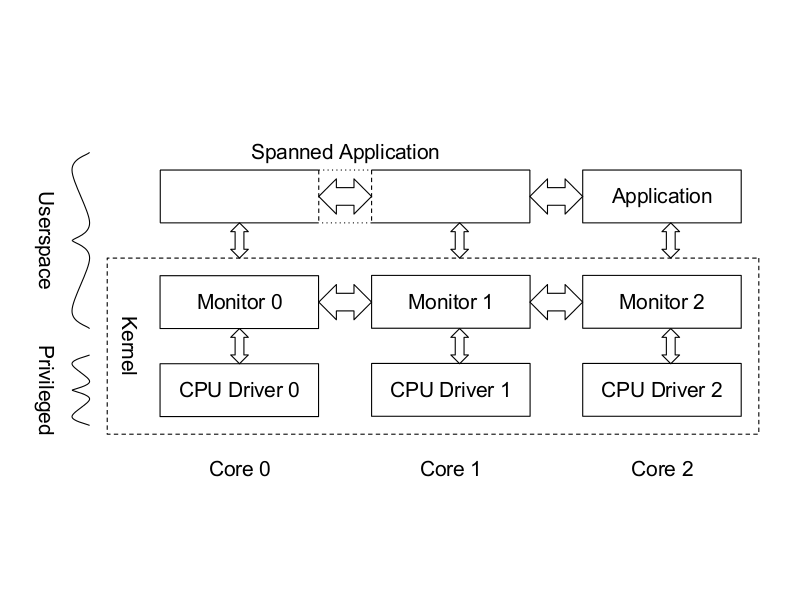
\includegraphics[scale=0.25]{img/BF_sharing_res}
\caption{Barrelfish Kernel Partitioning}
\label{kernelpartition}
\end{figure}
To manage resource utilization by the kernel, Barrelfish maintains an individual copy of the kernel on each core, and then performs synchronization to keep the system consistent. This is done to reduce the effort spent in synchronization, since the individual  copies have share-nothing policy by default. This design when extended to the userspace, creates a distributed system. This lets the system achieve the goal of running kernels on cores of different architectures in parallel. But it still faces the problems of low throughput and latency. The solution for this problem is to have a shared memory which does cache coherency, which requires certain communication channel between the cores to pass the capability information around. 

In Nevill and Rose, the authors have presented basic operations that can be performed when sharing of capability information is considered. The channels betweens cores maintain a send-once FIFO queue for sending messages containing these operations. Since sending and receiving these messages implies that there would be a need for synchronization between cores, there is a conflict which arises due to the fact that the initial goal was to maintain a synchronization-free system. The authors address this issue by considering object loyalty, which is that every capability object is assigned to an owning core. This ownership model is implemented along with certain defined invariants regarding the capability objects.~\cite{nevillmasters} Nevill and Rose also give preconditions and postconditions that must be met (as far as possible), to implement the Barrelfish capability operations.

We give a brief overview of the invariants, preconditions and postconditions below as mentioned in Nevill and Rose:~\cite{nevillmasters}

\begin{enumerate}
\item \textbf{Invariants:}
	\begin{itemize}
	\item \textbf{Ownership Property:} Every capability that is not Null has an \textit{owner} property that refers to a running kernel instance in the system.
	\item \textbf{Consistent Ownership:} Any two capabilities that are copies must have the same \textit{owner} property.
	\item \textbf{Owner Copies:} Every set of all copies of a capability must contain at least one capability where the owner matches the location. With other words, the owning core must always have a local copy.
	\end{itemize}
	
\item \textbf{Preconditions:}
\begin{itemize}
\item \textbf{Copy:} The source capability is not Null and the destination core is valid.
\item \textbf{Retype:} The source capability is not Null, may be retyped to the destination type, and has no descendants in the system.
\item \textbf{Delete:} The target capability is not Null.
\item \textbf{Revoke:} The target capability is not Null.
\end{itemize}

\item \textbf{Postcondition:}
\begin{itemize}
\item \textbf{Copy:} The destination core has a copy of the capability and the invariants of the system hold.
\item \textbf{Retype:} The specified descendants exist in the target slots and the invariants of the system hold.
\item \textbf{Delete:} The source capability is Null and the invariants of the system hold.
\item \textbf{Revoke:} All copies and descendants of the source capability have been deleted and the invariants of the system hold.
\end{itemize}
\end{enumerate}

These operations all refer to slots of memory. A slot is the storage required to store an individual capability, where a Null capability corresponds to an empty slot. As mentioned above, every slot has an owner as well as an immutable memory location. The slots are considered local if the owner and the memory location are the same, and foreign otherwise. The behaviour and interaction between these capability operations are described through global pseudocodes (for each operation), which we will not mention here due to space constraints.

Barrelfish's design has successfully applied aspects from an object oriented approach to a distributed, multi-core, many-core system. Though the authors have set out various optimizations as future scope and there are currently issues in the design regarding undelivered/unresponsive messages, it does lay out the basic groundwork for other capability based resource management systems to build on.

\section{Filesystems}
\label{sec:filesystem}

File systems are used to dictate how data is stored and retrieved, while traditionally file systems were designed for single system, although the advancements in distributed systems, gave rise to distributed file systems (often referred to as network file systems) which are now widely deployed. However one important concern, is the underlying access control mechanism for such a system, and capabilities are better suited\cite{miltchev2008} for this for a variety of reasons:
\begin{itemize}
\item ACLs (Access Control Lists) would be a bottleneck for a distributed system, since it requires explicit authentication whereas a user possessing a capability can access the resource listed in the capability with the rights specified in it.
\item capabilities explicitly list privileges over a resource granted to the holder and hence naturally support the property of least privilege
\end{itemize} 
While access control using capabilities sets the theme for access control in distributed file systems, their implementations vary vastly as seen by the implementation detail of two popular distributed file systems, OrangeFS and TahoeLAFS. While discussing these we limit ourselves to the capability aspect without addressing the other fundamental pillars of distributed file systems such as sharding and redundancy mechanisms.

\subsection{ OrangeFS }
OrangeFS emerged as a development branch of Parallel Virtual File System (PVFS2) in 2007, and tries to address applications for the future, one of which is secure access control. PVSF2 was designed with focus on performance for parallel applications sharing data across many clients for which it uses the notion of an 'intelligent server' architecture. OrangeFS being branched out of PVFS2 is build entirely in C itself like the latter.
%OrangeFS introduced capability based security only in November 2014

OrangeFS is an object based file system, where each file and/or directory has two (or more) associated objects to it, corresponding to the metadata and the actual file data (can be split into multiple objects). Storage nodes in OrangeFS usually provide two services
\begin{itemize}
\item Metadata Service: which sends and receives the metadata of directories and logical files (the actual data need not be stored on this node)
\item Data Servce : which sends and receives data for objects stored on this node.
\end{itemize}

On a high level, OrangeFS uses a certificate based security consists of two main parts, Authentication and Access Control, and like all contemporary file systems provides access control by determining a user's access to an object based on the object's ownership and permissions. Traditionally, secure systems have used certificates to cryptographically assure verifiable identity information in storable blocks of data, these certificates are generally associated with a private and public key pair, of which the public is generally stored in the certificate along with other fields significant to the application in consideration. In case of OrangeFS the key fields are :
\begin{itemize}
\item Issuer Distinguished Name: to identify the entity that issued and signed this certificate
\item Subject Distinguished Name(DN): identifies the user that the certificate authorizes
\item Validity Period: the duration for which this issued certificate is valid.
\end{itemize} 

\begin{figure}[h]
\centering
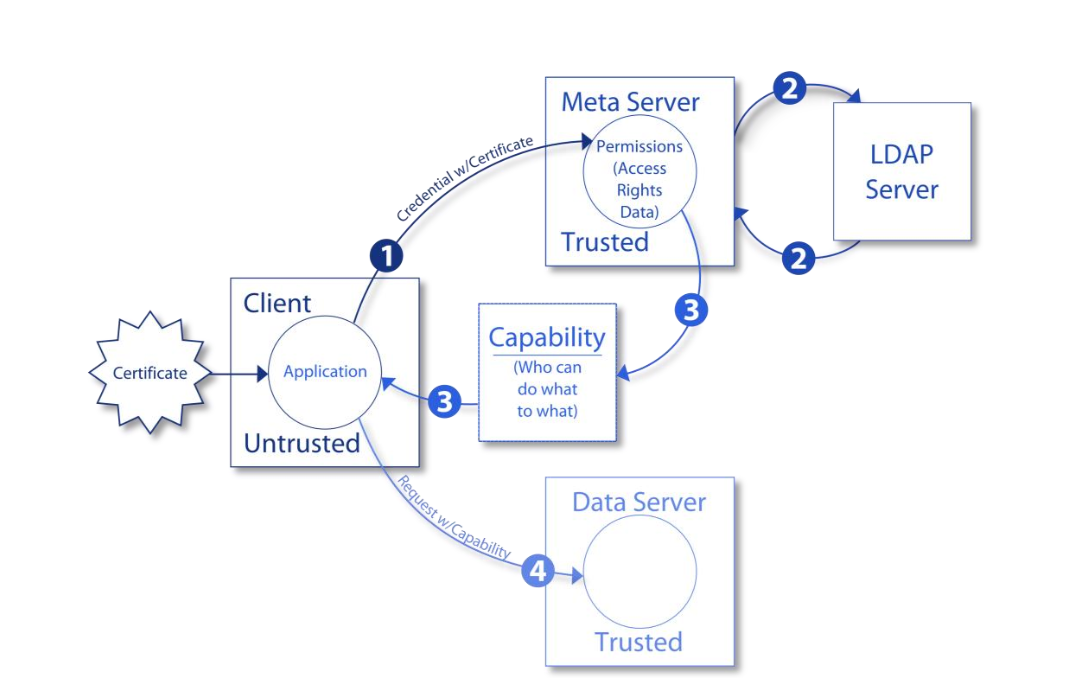
\includegraphics[scale = 0.2]{img/orange}
\caption{OrangeFS Architecture}
\label{orange}
\end{figure}

Another entity involved in this system, is the Lightweight Directory Access Protocol(LDAP) directory which stores user objects (such as UID and GID to evaluate access rights). The Subject DN from the certificate is used to uniquely identify users in LDAP directory, and OrangeFS servers interact with LDAP servers to obtain the user information to enforce the desired access control. 

In every system that makes use of certificates for security must have a root(or roots) of trust, which can be used to issue valid certificates for other entities in the system. In OrangeFS, the trusted root certificate is called a Certificate Authority(CA) certificate, and is securely stored across each OrangeFS servers to sign and validate user certificates. Every user must have a valid user certificate (and the corresponding private key to the public key signed in their certificate) which is signed by the CA certificate. OrangeFS uses the term credential for a signed user certificate, and capabilities are signed objects containing permissions for file system objects.

As seen in Fig. \ref{orange}, capability based access control can be explained in a 4 step process:
\begin{enumerate}
\item To perform a request, client sends its credential along with request to the server.
\item Server verifies credentials signature and fetches corresponding user information from the LDAP server for the subject DN in the user certificate. 
\item Server compares the user permissions with the object permissions and constructs a capability for the request.
\item Client can use the capability to act on the file system object
\end{enumerate}
One aspect to notice is that all the secure components are created with an expiration period, since revocation in a system based on capabilities can go in either two directions, by basing itself on revocation through time outs, or by using a central entity that performs revocations but there introducing a bottleneck again.

\subsection{TahoeLAFS}
One fundamental difference of TahoeLAFS(Least Authority File System) from OrangeFS is that it assures 'provider-independent security', implying that the server itself which provides the file system does not have the ability to read or modify the data, hence reducing quite a lot of latent security issues that arise from a compromised server. Moreover this bolsters their claim of true 'least-authority' semantics. This guarantee is integrated naturally into the implementation mechanism of Tahoe-LAFS and requires no additional step or management. 

TahoeLAFS\cite{tahoelafs} considers two kinds of files : mutable and immutable, and provides its access control mechanism with this in consideration. Any file uploaded to the storage grid can be chosen as either kind, and any user who has read-write access to a mutable file or directory can give other users read-write access or even any diminishing subset of the capabilities owned by the user. 

Irrespective of the type of file, all files in TahoeLAFS undergo erasure coding using Reed-Solomon codes, which allows a write to split a file into N share out which K shares need to be used to read (however Tahoe maintains small numbers for both K and N thus maintaining low computational costs for erasure coding)

\begin{figure}[h]
\centering
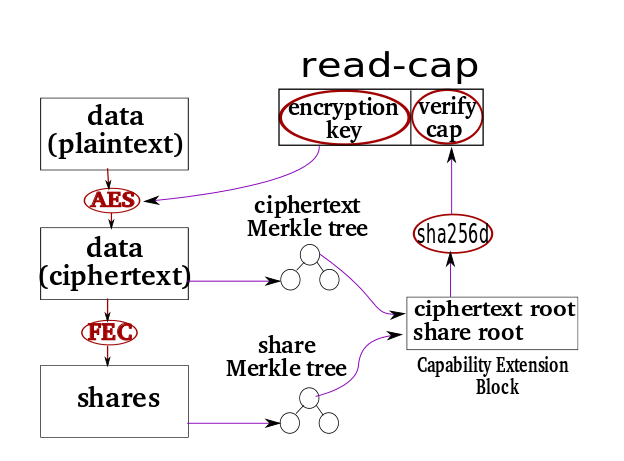
\includegraphics[scale = 0.2]{img/immutable}
\caption{Immutable Files in TahoeLAFS}
\label{immutable}
\end{figure}

In TahoeLAFS, each immutable file has two associated capabilities, the read capability called as the \textit{read-cap} and verify capability or 
\textit{verify-cap}. To create an immutable file, the client chooses a symmetric encryption key to encrypt the file which it loads on the server. The verify-cap is derived from the ciphertext of the file using a secure hash (SHA256d\footnote{SHA256d(x) = SHA256(SHA256(x)) (to prevent length-extension attacks double SHA hashing is performed}). However verification has two problems to be taken care of
\begin{itemize}
\item If integrity check fails, client needs to isolate the erasure code shares that were wrong, for which a Merkle tree is constructed over the erasure code shares, allowing client verification of each share involved.
\item However just the Merkle Tree over erasure code shares is not sufficient as that does not link the shares to the original file content\footnote{the creator of the file could generate erasure code shares from two different files and use the shares from both in the set of N shares covered by the Merkle Tree, resulting in a different file depending on the subset of shares used to reconstruct}, and hence another Merkle Tree is constructed over the ciphertext itself.
\end{itemize}
Now, as seen in Fig.\ref{immutable} the roots of both the Merkle Trees are kept on each server alongside the shares, and is called as the 'Capability Extension Block' \footnote{Logically should be part of the capability but maintained on the servers to minimize capability size}. The verify-cap is now the secure hash of the Capability Extension Block, and the read-cap to an immutable file is the verify-cap along with the original symmetric encryption key. Thus allowing the clients with the read-cap to simply pass on the verify-cap component to other clients when it wants to give it a diminished form of it's capability, moreover since the file is encrypted with the symmetric key prior to storing on to the servers, the servers themselves cannot read the data, and any attempts to modify would break the integrity check done by the verify-cap.
%footnote about choosing key can be based on the hash of plaintext of the file - convergent encryption

\begin{figure}[h]
\centering
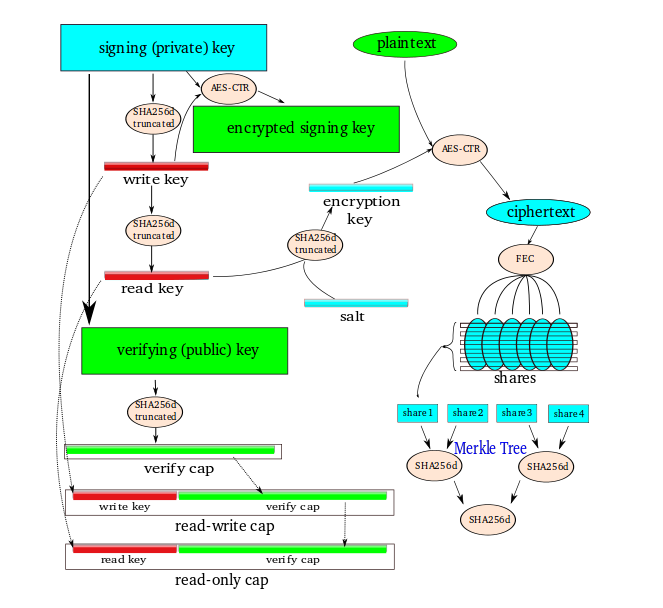
\includegraphics[scale = 0.2]{img/mutable}
\caption{Mutable Files in TahoeLAFS}
\label{mutable}
\end{figure}

For mutable files the underlying process is significantly different and more convoluted to take care of the three desired capabilities \textit{read-write-cap}, textit{read-only-cap} and \textit{verify-cap}. Each mutable file is associated with an RSA key pair( with private key SK), a client first computes the write key, WK = SHA256d(SK) and corresponding read key, RK = SHA256d(WK). To write, a client generates a new 16 byte salt, and computes the encryption key with EK = H(RK,salt). A similar process for integrity verification is performed over the ciphertext, by computing a Merkle Tree over the erasure coded shares of the ciphertext, and the client signs the root hash of the Merkle Tree as well as the salt, with the private key SK. So the verify-cap for mutable files are the secure hash of verifying key : VC = SHA256d(VK), hence allowing clients with verify-cap to check that the verifying key which is stored on the server is the right one. The read-only cap to a mutable file include VC, and the read key RK(RC = VC,RK), while the read-write-cap to a mutable file includes VC and the write key WK (WC = VC,WK). However the owners of read-write-cap still need to be able to produce digital signatures on new versions for which the signing key SK is stored on the server encrypted with WK which is only available to the clients with read-write-cap. 

A directory could simply be treated as a mutable file which contains a set of tuples of <child name, capability to child>, this allows anyone given read access to a directory to be able to learn the child names and corresponding read capabilities, and similarly for read-write capabilities as well as for mixed capabilities for individual files of the directory. However, Tahoe implements transitive read-only access to directories, i.e. directories which have read-only access to the directory can get only a read-only-cap to a child. For this, directory includes two slots for the caps for each child, and read-write-caps for the children are encrypted separately before being stored in the mutable file.

\subsection{Comparison}
It becomes clear from the above two sections that TahoeLAFS and OrangeFS, while use the same abstraction of capability based access control mechanisms, they are entirely different in their implementation, while OrangeFS reflects a capability system with tag bits, Tahoe's implementation is based on the password/sparse capability system. Even the security properties and guarantees offered by them are different, the most significant contribution this being the notion of provider-independent security introduced in TahoeLAFS. There are many other subtle implementation details that make them highly incomparable against each other, such as the erasure coding in TahoeLAFS allows different subsections of files to be loaded from different servers, thus improving performance by improving parallelism. Moreover OrangeFS is a completely build from C, whereas TahoeLAFS is implemented in Python. Another aspect is the revocation of capabilities, while OrangeFS relies on time outs to perform revocation, in case of Tahoe since the key once given cannot be revoked, the only option is for a client to redistribute a new set of capabilities under new keys for an object, which is a significantly costly process. Hence in short, evaluating the performance of these two types of systems would not provide any insightful results.




\hfill
\section{User Space implementations}
There also is some work done in the area of capability based resource management in the user space. We now describe two such systems. 
	\subsection{Capsicum}
\label{subsec:capsicum}
%<Kritika>

Capsicum is one user space implementation for a capability based access control system developed at the University of Cambridge Computer Laboratory. \footnote{https://www.cl.cam.ac.uk/research/security/capsicum/} It is a lightweight framework that extends the POSIX API. It implements capabilities by modifying current kernel primitives as well as by performing sandboxing techniques in the userspace. It provides capabilities for logical applications by implementing \textit{compartmentalization} of the application. The first implementation for Capsicum was on FreeBSD 8.x, and as a result of more research being conducted, it is now being released along with FreeBSD 9.0 as an experimental feature.

The implementation of capabilities by extending, rather than gives the applications the benefit of having least-privilege operations in the system. Separation or compartmentalization is a popular technique used by OSs today to help security-critical applications in dealing with vulnerabilities. It limits the impact of the system by exposing only a small part or compartment of the entire system to the vulnerability.The other critical aspect of implementing such a system is to make sure that this is achieved by minimum effort.

Capsicum achieves this by implementing certain security primitives like \textit{capability mode} and \textit{capabilities.} Some of the implementation modifies the kernel level primitives, while others are for userspace implementation. These primitives together support logical compartmentalization of the application. Once the application code is separated into individual logical parts, we can run independent sandboxes to form logical applications as shown in Figure \ref{compartment}.

\begin{figure}[h]
\centering
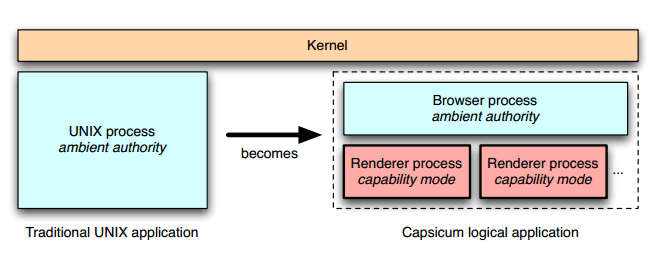
\includegraphics[scale=0.45]{img/capcisum_sandbox}
\caption{Logical compartmentalization of applications}
\label{compartment}
\end{figure}

Following is the list of all such primitives:

		\begin{itemize}
		    \item \textbf{capabilities:} file descriptors with refined privileges.
   		    \item \textbf{capability mode:} implementing sandboxing so as to deny access to global namespaces.
    		    \item \textbf{process descriptors:} replacing capability-centric process IDs. 
    		    \item \textbf{anonymous shared memory objects:} an extension to the POSIX shared memory API.
    		    \item \textbf{rtld-elf-cap:} constructing sandboxed applications from run-time linkers by modifying ELF 
    		    \item \textbf{libcapsicum:} library to create and use capabilities components
    		    \item \textbf{libuserangel:} library allowing sandboxed applications or components to interact with user angels, such as Power Boxes.
    		    \item \textbf{chromium-capsicum:} Google's Chromium web browser that provides effective sandboxing of high-risk web page rendering.

		\end{itemize}
		
Capsicum has a host of capability implementation that can be used, but they leave the end user to use his/her discretion in order to maximize the security impact for their respective application. Implementing the \textit{capability mode} for example, implies that a process flag is set by the system call. Once this flag is set, the system goes into the capability mode, and the process is then denied access to global namespaces. In addition to this, in the capability mode, the access to the certain system calls is also limited.

In Capsicum, capabilities can also be implemented using file descriptors. File descriptors have certain properties that are considered desirable in a capability system, like being a tokens of authority, being unforgeable as well as being able to pass the properties through inheritance. In Capsicum, the \textit{cap\_new} system call extends the file descriptor by creating a new capability and a set of rights. These rights get checked by \textit{fget} which performs the conversion of file descriptor  arguments to system calls to in-kernel references.
	\subsection{capBAC}
\label{subsec:capbacsystem}
<Sajin>




\section{implementation and results}
\label{sec:implementation}
<k,j,s>


\section{Conclusion}
\label{sec:conclusion}
<k,j,s>


\bibliographystyle{abbrv}
\bibliography{bib}

%\balancecolumns 

\end{document}
